\begin{figure*}[t]
\centering
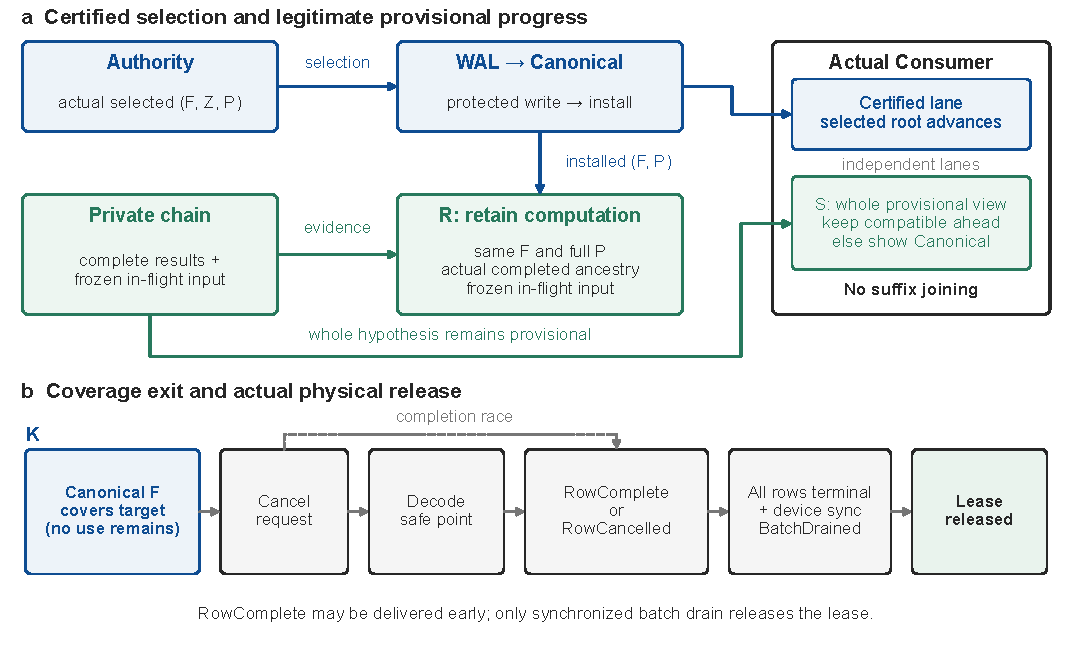
\includegraphics[width=\textwidth]{figures/coordination_protocol.pdf}
\caption{RevTrace coordinates complete provisional computation and whole
Consumer views with certified state. $R$ and $S$ use the same declared
feedback dependencies, with separate sufficient guards. Coverage retirement
uses a different predicate. A complete result may be consumed before its
batch drains; only terminal rows plus device synchronization release the
physical lease.}
\label{fig:protocol}
\end{figure*}

\subsection{Complete results and physical ownership}
This section describes the core ASR runtime. The native correction adapter
uses its separately declared full-state interface; its validation does not
inherit the core kernel's recovery or physical-lease evidence automatically.
Figure~\ref{fig:protocol} separates publication from physical completion.
Each dispatch binds a session, worker incarnation, job, frozen input, target
frontier, and execution contract. The wrapper accepts only an exclusive
complete-row or cancelled-row outcome. It re-derives feedback state and
text from the bound complete result. A cancelled row reports accounting
information and supplies no partial feedback state.

The Owner can validate, durably install, and publish a complete row while
other rows of its physical batch are still running. This prevents a
completed session from inheriting another row's entire completion delay.
Physical ownership has a separate condition: every row must have a terminal
outcome and the device must synchronize before \texttt{BatchDrained}
releases the batch lease. A complete publication alone cannot authorize
reusing the executor.

\subsection{Covered work and safe-point exit: \texorpdfstring{$K$}{K}}
An old birth version does not determine either usability or uselessness.
For the tested use model, $K$ requests exit when the actually installed
Canonical frontier covers a proposal's target and that work has no
remaining declared use. This coverage predicate answers a different question
from $R$: a valid continuation beyond the new root may still be useful.

\texttt{CancelRequest} is a request, not a completion event. The worker
observes it at supported decode boundaries. Completion can win the race;
the runtime records either a complete result or cancellation, never both.
It waits for all row terminals and actual drain before releasing the lease.
The static batch is not compacted or refilled, and residual cost for masked
rows remains in the measurements. The protocol supplies no arbitrary-GPU
millisecond cancellation guarantee. Its service value is the measured
execution window available to subsequent lawful work.

\subsection{Durable facts and outstanding input}
Canonical state and transition identity are synchronized before a successful
acknowledgment. Each journal frame binds the parent and next state, request
identity, selected complete result, and receipt. The runtime verifies that
the recorded delta reconstructs the proposed state. Group-ready commit
shares a synchronization barrier among already validated transitions of
different sessions; it introduces no collection timeout and no cross-session
all-or-nothing transaction. An uncertain append or state-application outcome
blocks further writes until recovery.

Recovery validates framing, checksums, state chaining, and contracts, then
reconstructs certified state and admitted identities. An identical retry
retrieves its recorded outcome; a changed request with the same identity
conflicts. These are conventional write-ahead recovery principles
\cite{mohan1992aries} instantiated at the feedback boundary.

In the recovery configuration, the recovered view can be applied before cold neural workers finish
loading. This restores existing service facts, not progress on new audio.
The input journal separately preserves accepted but uncertified audio and
its original clocks, so replaying old text cannot discharge new work.
Process epochs fence old workers and publications. These checks rely on
exclusive ownership and intact synchronized storage, as declared in
Section~\ref{sec:contract}.

\subsection{Validation boundaries}
The re-rooting argument and conditional view property are supported by
targeted source-level witnesses and actual service interleavings.
Separately, bounded exploration of an earlier recovery prototype covers
durable-root, view-application, and physical-lease interleavings. Its
1,154-state single-session product does not represent the full multi-node
re-rooting guard or an arbitrary neural execution. We therefore use it as
component-level protocol evidence, with its own frozen source, rather than
a complete machine proof of Propositions~\ref{prop:rebase}
and~\ref{prop:continuity}.

A separately frozen recovery prototype completed 84 GPU service runs:
24 normal, 36 process-group SIGKILL, 16 controlled-boundary, and eight
post-sync crashes. The 44 crash audits recorded no acknowledged-input loss.
All 32 early-recovery crash runs reapplied old facts before workers were
ready. In one Qwen configuration, median old-view recovery changed from
31.013 to 14.736~s; first new certified output still took 33.829~s.
The complete-composition control shared the benefit. All 44 crash runs
missed whole-run D2/C8. These are earlier-prototype measurements, not fault
validation of the current core or native adapter.
